\section{Resultados e discussões}
\subsection{Figuras de Chladni}

\subsection{Tubo de Rijke}

\subsection{Diapasão e coluna d'água}
O experimento do diapasão com coluna de água é uma demonstração clássica da física ondulatória, utilizada para estudar os princípios da ressonância em tubos fechados. No dito experimento, ao colocar diferentes diapasões com frequências diferentes e conhecidas na boca do tubo, fez com que as ondas sonoras se propagassem pela coluna de ar dentro do tubo sendo refletido pelas paredes até a extremidade superior da água, que reflete a onda. 

Para cada diapasão diferente testou-se que, ao variar o nível da água no tubo por completo, ou seja, varia-lo do menor ponto até o maior ponto, observou-se que, em pelo menos um ponto, houve um grande aumento na intensidade sonora, e esse ponto foi demarcado com a descrição da frequência do diapasão que foi usado. Para o melhor tratamento e análise de dados, será aprofundada a discussão quanto aos dados obtidos com o experimento com o diapasão de \qty{512}{Hz}, que poderá ser abrangida para os testes com os outros diapasões.

O experimento com o diapasão de \qty{512}{Hz} apresentou dados singulares, sendo o único que apresentou dois pontos onde houve um grande aumento na intensidade sonora.  Esses dois pontos foram marcados e tiveram suas colunas de ar medidas, como mostrado na \cref{TuboFechado}.
\begin{figure}[H]
	\centering
	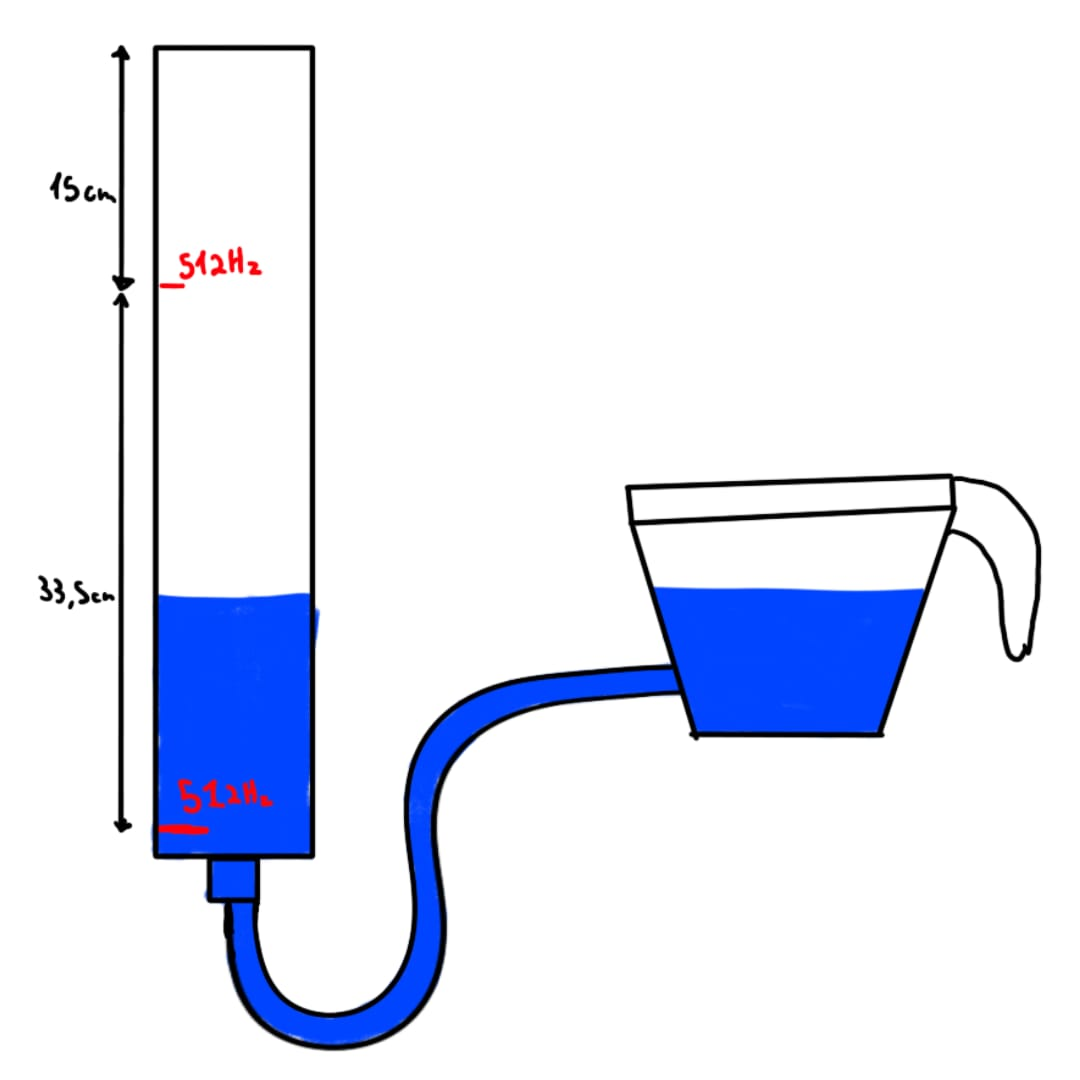
\includegraphics[width=0.35\linewidth]{fig/TuboFechado.png}
	\caption{Tubo de água com uma extremidade fechada e sistema de modificação do nível, marcados e medidos os pontos em que houveram um aumento significativo na intensidade sonora com a vibração de um diapasão de \qty{512}{Hz}. Fonte: Autoria própria.}
	\label{TuboFechado}
\end{figure}

Esse aumento significativo na intensidade do som, ocorre pois quando a onda se propagou pela coluna de ar dentro do tubo, e refletiu-se pela extremidade fechada (superfície da água), criou-se uma \textit{onda refletida} com defasagem de 180º para a onda original, e essa interferência entre as ondas incidentes e refletidas deu origem a uma onda estacionária. Essas ondas estacionárias, são os modos normais de vibração da coluna de ar contida no tubo, que possuem seus pontos de ressonância identificáveis por um aumento significativo na intensidade sonora. E em um tubo com uma extremidade fechada, esses pontos de ressonância ocorrem quando o comprimento da coluna de ar (\(l\)) corresponde a \(\frac{\lambda n}{4}\), para valores impares de n, com n natural, como demonstrado pela imagem \cref{NodoEAntinodo}. 

\begin{figure}[H]
	\centering
	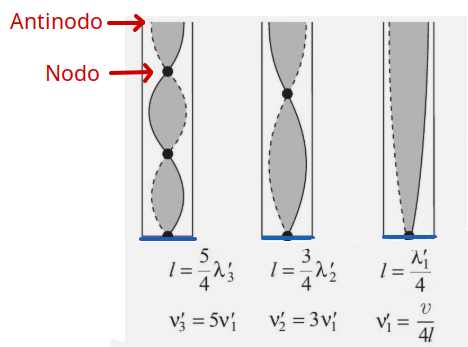
\includegraphics[width=0.35\linewidth]{fig/NodoEAntinodo.png}
	\caption{Demonstração da interferência entre ondas incidentes e refletidas em um tubo fechado, com a formação de nodos e antinodos, posicionados na extremidade fechada e na extremidade aberta, respectivamente, quando as ondas encontram um ponto de ressonância. Abaixo da imagem, formulas de demonstração do tamanho da coluna de ar em que o ponto de ressonância é identificado. Fonte: Modificação de imagem do livro Moyses vol 2.}
	\label{NodoEAntinodo}
\end{figure}

Segundo os dados retirados do experimento, sabe-se que os pontos de ressonância das ondas estacionarias ocorreram com uma coluna de ar de tamanhos \qty{15}{cm} e \qty{48,5}{cm}, possibilitando o calculo do comprimento da onda referente ao primeiro harmônico, que ocorre ao menor \(l\).

\begin{align*}
	l &= \frac{\lambda}{4}\\
	\qty{15}{cm} &= \frac{ \lambda}{4}\\
	\lambda &= \qty{60}{cm} = \qty{0,6}{m}
\end{align*}

Dessa forma, como possui-se o comprimento de onda do som \(\lambda\), e a frequência da onda \(f\), é possível calcular-se a velocidade do som no ar:

\begin{align*}
	v &= \lambda \cdot f\\
	v &= \qty{0,6}{m} \cdot \qty{512}{Hz} \\
	v &= \qty{307,2}{m/s}
\end{align*}

Os resultados experimentais indicaram uma velocidade do som de \qty{307,2}{m/s}, apresentando uma diferença de aproximadamente 10,4\% em relação ao valor teórico de \qty{343}{m/s}. Esta discrepância pode ser atribuída principalmente a: (1) variações nas condições ambientais (temperatura e umidade), já que a velocidade do som varia com a temperatura do ar; (2) imprecisões na determinação do ponto exato de ressonância; e (3) possíveis erros sistemáticos nas medições. Apesar da diferença, o experimento demonstrou ser um método válido para estimativa da velocidade do som em condições controladas.

\subsection{Experimento de Uma Corda}
Este experimento ilustra o princípio de funcionamento dos instrumentos de corda, nos quais o som é produzido pela vibração das cordas. Ao serem colocadas em oscilação, as cordas perturbam o meio ao seu redor, gerando ondas sonoras — variações de pressão que se propagam pelo ar. O perfil dessa oscilação determina as características da onda sonora gerada. Assim, ao alterar propriedades como a frequência ou o comprimento da onda, modifica-se o som produzido.

No experimento de uma corda, observou-se a variação do som emitido pela vibração da corda ao alterar a tensão da mesma. Observando mais especificamente, quando aumentada a tensão da corda, adicionando mais peso a sua extremidade livre, foi possível obter um som mais agudo, ou seja, uma frequência maior.

A explicação dessa alteração de som é sustentada pelas leis das Cordas Vibrantes, descritas por Mersenne. Mais especificamente pela sua segunda lei, que diz, que a frequência fundamental de uma corda é proporcional à raiz quadrada de sua tensão, ou seja, ao aumentar a tensão, aumenta-se sua frequência, e produz um som mais agudo. 

Dessa forma, foi explicado o porquê intrumentos de corda são afinados aumentando a tensão de suas cordas, porém, as leis de mersenne tambpém explicam o porque nesses instrumentos existe a presença de múltiplos tipos de cordas. Segundo as leis de Mersenne, a produção de diferentes sons, a partir de uma corda, pode ser controlada através de três parâmetros principais: (1) a tensão aplicada, (2) o comprimento da corda e (3) suas propriedades físicas. Como o comprimento é limitado pela estrutura do instrumento e a tensão máxima pela resistência do material, a terceira lei de Mersenne oferece uma solução prática: a frequência fundamental é inversamente proporcional à raiz quadrada da densidade linear. Assim, variando a espessura e o material das cordas - e consequentemente sua densidade linear - é possível expandir significativamente a faixa tonal do instrumento. Este princípio é particularmente evidente em guitarras, onde cordas de diferentes calibres (mais finas para agudos, mais grossas para graves) permitem a execução de notas em diversas oitavas.
